\documentclass{beamer}
\usetheme{CambridgeUS}
\usefonttheme{structuresmallcapsserif}
\usecolortheme{beaver}
\usepackage[utf8]{inputenc}
\usepackage[portuguese]{babel}
\usepackage{amsmath,amsthm,amsfonts,amssymb,dsfont,mathtools}
\usepackage{graphicx,xcolor,enumerate}
\usepackage{indentfirst}
\usepackage{array}
\usepackage{tabularx}
\usepackage{hyperref}
\usepackage{tikz}

%-------------------- CAPA ---------------------------------------
\title[Science Challenge 4A]{Coexistência e Compartilhamento Dinâmico de Espectro em Comunicações Móveis 6G} 
\subtitle{\textit{Adaptive Beamforming e Controle de Potência}} 
\author[M. Camelo, C. Rodrigues]{Mikael Ribeiro Camelo\inst{1} \and Caio Rodrigues\inst{1}} 
\institute[UFC]
{\inst{1}
Universidade Federal do Ceará\\Centro de Tecnologia\\Departamento de Teleinformática\\ \vspace{0.15cm} Prof. F. Rodrigo P. Cavalcanti} 
\date{2026.2} 

\AtBeginSection[]
{
  \begin{frame}
    \frametitle{Sumário}
    \tableofcontents[currentsection, hideallsubsections]
  \end{frame}
}

\begin{document}

\begin{frame}
    \titlepage
\end{frame}

\begin{frame}{Sumário}
    \tableofcontents[hideallsubsections]
\end{frame}

% ======================================================= %
% SEÇÃO 1: ATIVIDADE 1 - BEAMFORMING E DUAL-LOOP PC
% ======================================================= %
\section{Atividade 1: Otimização Conjunta de Beamforming e Controle de Potência} 

\begin{frame}{Acoplamento e Estratégia \textit{Dual-Loop}} 
    Investigação do acoplamento entre a filtragem espacial via \textit{Adaptive Beamforming} com MRC e DPC em uma topologia multicelular (16 APs)

    \vspace{0.2cm}
    \begin{columns}
        \begin{column}{0.48\textwidth}
            \textbf{Arquitetura em Malha Dupla:} 
            \begin{itemize}
                \item \textbf{Limitação do DPC Fixo ($\gamma_{\text{tar}} = 10\text{ dB}$):} Subutiliza o ganho direcional em enlaces favoráveis. 
                \item \textbf{Malha Interna (Rápida):} Atualiza iterativamente a potência $p_k$ buscando a meta local $\gamma_{\text{tar},k}$. 
                \item \textbf{Malha Externa (Lenta):} Ajusta dinamicamente o alvo $\gamma_{\text{tar},k} \in [-10, 20]\text{ dB}$ (iniciando em $10\text{ dB}$). 
            \end{itemize}
        \end{column}
        
        \begin{column}{0.52\textwidth}
            \begin{block}{Regras de Negociação de Alvo (\textit{Outer Loop})} 
                \begin{enumerate}
                    \item \textbf{Aumento ($+1\text{ dB}$):} Se o UE atinge a meta com $p_k < p_{\max}$, sobe até o teto QAM de $20\text{ dB}$. 
                    \item \textbf{Redução ($-1\text{ dB}$):} Se satura em $p_k = 1\text{ W}$ e $\gamma_k < \gamma_{\text{tar},k}$, alivia a CCI nas células vizinhas. 
                    \item \textbf{Bloqueio (\textit{Outage}):} Se $\gamma_{\text{tar},k} < -10\text{ dB}$, desliga o transmissor ($p_k = 0$). 
                \end{enumerate}
            \end{block}
        \end{column}
    \end{columns}
\end{frame}

\begin{frame}{Análise Comparativa de KPIs (Exercício 1)} 
    Desempenho do \textbf{Dual-Loop PC} frente aos cenários \textbf{Full Power ($1\text{ W}$)} e \textbf{DPC Fixo ($10\text{ dB}$)} sob realizações idênticas de canal (mesma \textit{seed}). 

    \vspace{0.15cm}
    \begin{table}
        \centering
        \resizebox{0.98\textwidth}{!}{
        \begin{tabular}{c|l|cccc}
            \hline
            \textbf{Carga ($K$)} & \textbf{Algoritmo} & \textbf{Border SE (10º Pct)} & \textbf{Sum-Capacity SE} & \textbf{Eficiência Energética} & \textbf{Taxa de Outage} \\ 
            & & \textbf{[bps/Hz]} & \textbf{[bps/Hz]} & \textbf{[Mbits/Joule]} & \textbf{[\%]} \\ 
            \hline
            $K = 1$ & Full Power (1W)         & 1.05 & 3.84 & 384.03 & 0.26\% \\ 
            $K = 1$ & DPC Fixo (Meta 10 dB)   & 1.05 & 2.77 & 446.89 & 0.26\% \\ 
            $K = 1$ & Dual-Loop PC (Outage)   & 0.96 & 3.50 & \textbf{465.40} & 0.34\% \\ 
            \hline
            $K = 4$ & Full Power (1W)         & 0.73 & 14.37 & 359.14 & 2.06\% \\ 
            $K = 4$ & DPC Fixo (Meta 10 dB)   & \textbf{0.85} & 10.67 & 412.89 & \textbf{0.73\%} \\ 
            $K = 4$ & Dual-Loop PC (Outage)   & 0.72 & 14.23 & \textbf{434.99} & 1.58\% \\ 
            \hline
            $K = 8$ & Full Power (1W)         & 0.45 & 26.44 & 330.48 & 4.32\% \\ 
            $K = 8$ & DPC Fixo (Meta 10 dB)   & \textbf{0.66} & 20.28 & 374.74 & \textbf{1.50\%} \\ 
            $K = 8$ & Dual-Loop PC (Outage)   & 0.48 & \textbf{26.38} & \textbf{406.27} & 3.29\% \\ 
            \hline
        \end{tabular}}
    \end{table}

    \vspace{0.1cm}
    \footnotesize{
    \begin{itemize}
        \item \textbf{Recuperação de Capacidade:} Em $K=8$, o DPC Fixo perde $23.3\%$ de \textit{Sum-Capacity} ($20.28\text{ bps/Hz}$), enquanto o \textit{Dual-Loop} alcança $26.38\text{ bps/Hz}$ (empatando com \textit{Full Power}). 
        \item \textbf{Eficiência Energética:} Liderança absoluta do \textit{Dual-Loop} em todas as cargas ($406.27\text{ Mbits/Joule}$ em $K=8$) ao evitar desperdício acima de $20\text{ dB}$ e desligar UEs inviáveis. 
    \end{itemize}}
\end{frame}

\begin{frame}{Comportamento Físico dos KPIs Primários} 
    \begin{columns}
        \begin{column}{0.44\textwidth}
            \textbf{Destaques em Alta Carga ($K=8$):} 
            \begin{itemize}
                \item \textbf{Ganhos sobre \textit{Full Power}:} O \textit{Dual-Loop PC} eleva a \textit{Border SE} ($0.48$ vs. $0.45\text{ bps/Hz}$) e reduz o \textit{Outage} de $4.32\%$ para $3.29\%$. 
                \item \textbf{DPC Fixo na Borda:} Atinge maior \textit{Border SE} ($0.66\text{ bps/Hz}$) e menor \textit{Outage} ($1.50\%$), mas sacrifica quase $1/4$ da capacidade agregada da rede. 
                \vspace{0.50cm}
                
            \end{itemize}
        \end{column}
        
        \begin{column}{0.56\textwidth}
            \begin{center}
                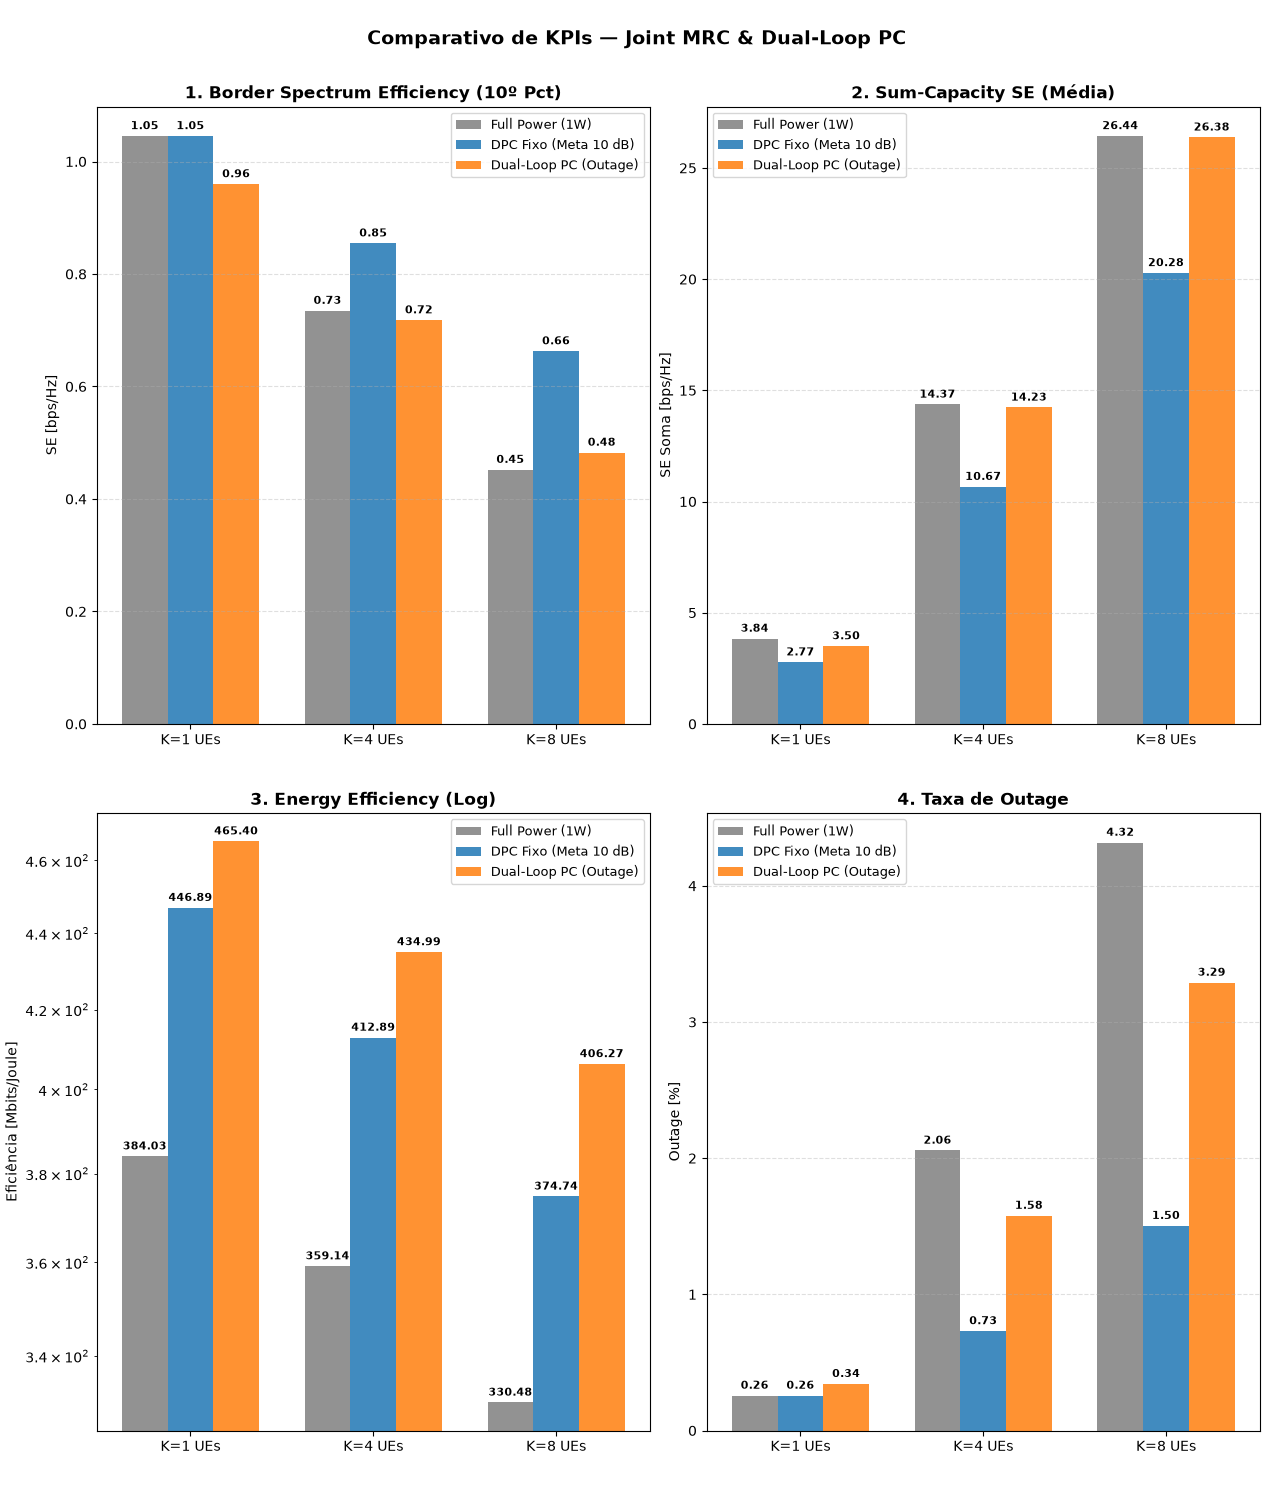
\includegraphics[width=0.95\linewidth]{Imagens/Activity01.png} %
                \\ \footnotesize{\textit{Comparativo dos 4 KPIs primários para $K \in \{1, 4, 8\}$ UEs.}} 
            \end{center}
        \end{column}
    \end{columns}
\end{frame}

\begin{frame}{Análise Estatística das CDFs} 
    \begin{columns}
        \begin{column}{0.44\textwidth}
            \begin{itemize}
                \item \textbf{CDF de Potência:} Curvas em degraus mostram que mais de $50\%$ dos UEs operam abaixo da potência máxima ($0\text{ dBW}$). 
                \item \textbf{CDF de SINR:} O DPC Fixo trava em um degrau vertical em $10\text{ dB}$, enquanto o \textit{Dual-Loop} avança até $+20\text{ dB}$. 
                \item \textbf{CDF de Capacidade:} Com o teto QAM em $20\text{ dB}$, o \textit{Dual-Loop} sobrepõe-se ao \textit{Full Power} nos percentis superiores poupando energia. 
            \end{itemize}
        \end{column}
        
        \begin{column}{0.56\textwidth}
            \begin{center}
                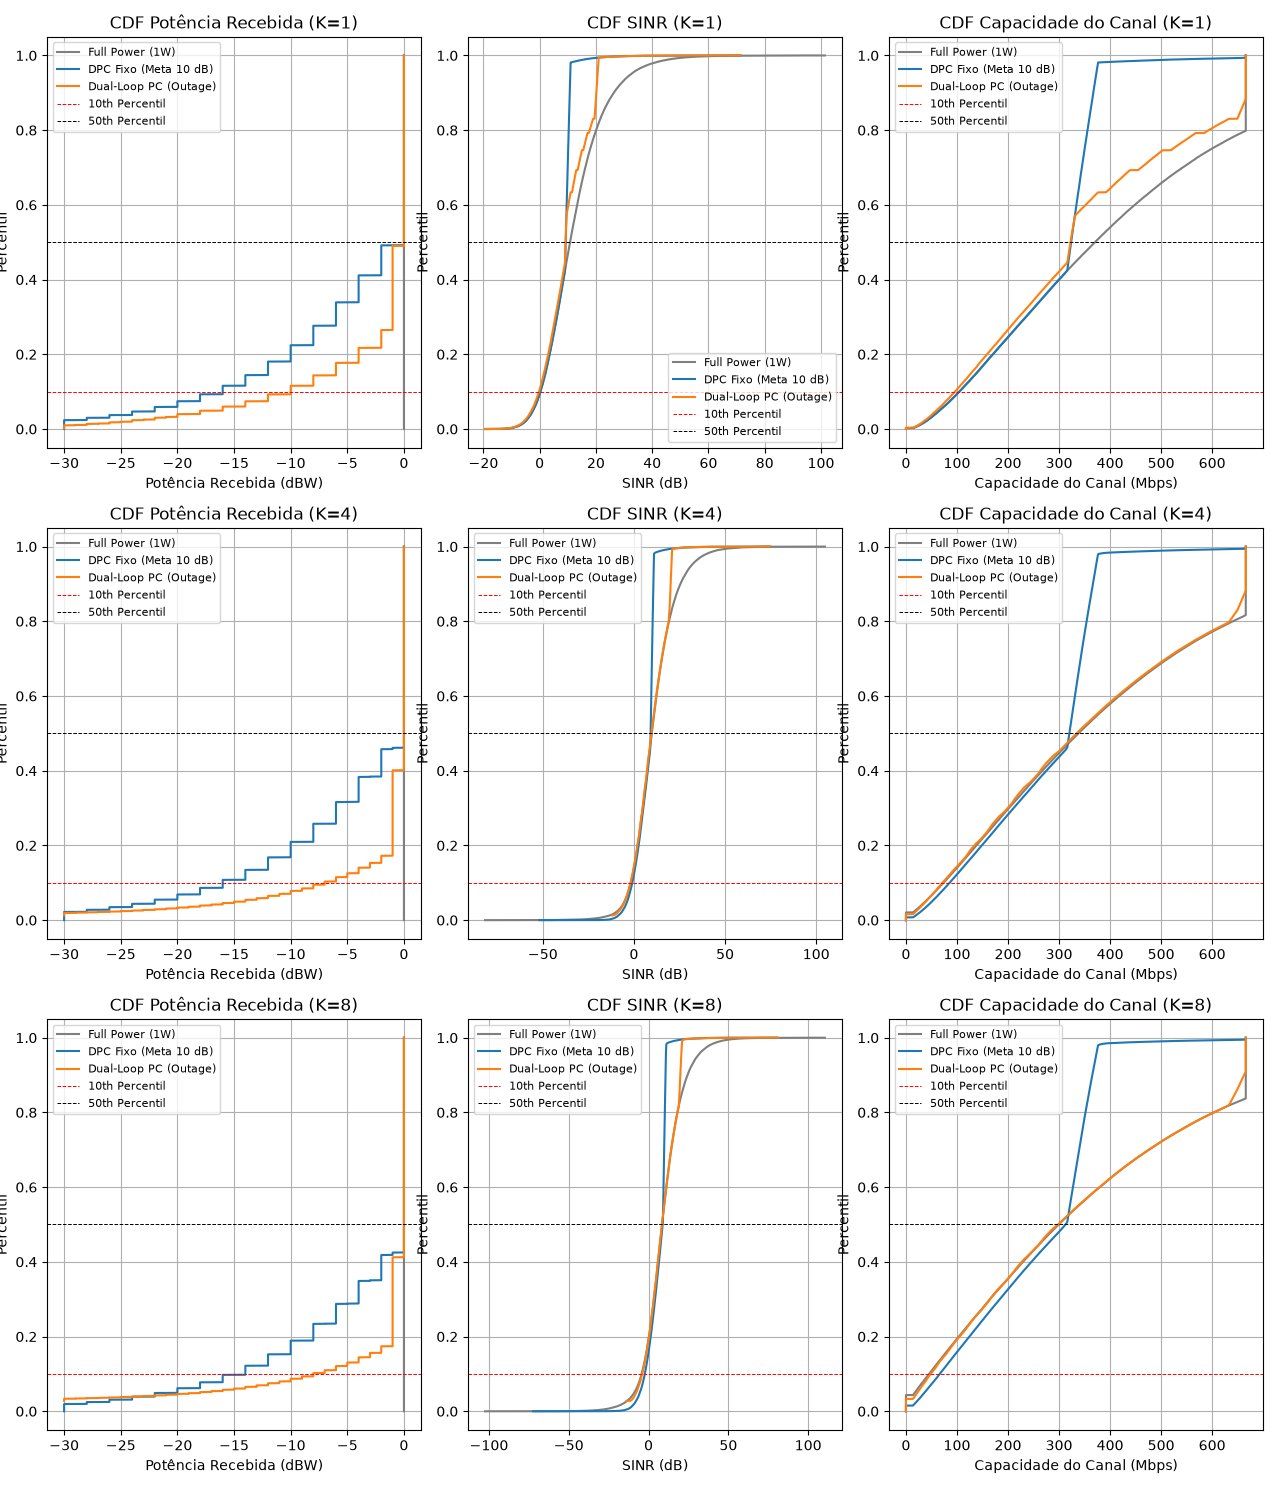
\includegraphics[width=0.95\linewidth]{Imagens/Activity01A.png} %
                \\ \footnotesize{\textit{CDFs empíricas para $K \in \{1, 4, 8\}$ UEs.}} 
            \end{center}
        \end{column}
    \end{columns}
\end{frame}

% ======================================================= %
% SEÇÃO 2: ATIVIDADE 2 - IMPACTO DA MOBILIDADE NO BEAMFORMING
% ======================================================= %
\section{Atividade 2: Impacto da Mobilidade no Desempenho do Beamforming} 

\begin{frame}{Modelagem Cinemática, ULA e Atraso de Rastreamento} 
    Transição para simulação dinâmica orientada ao tempo ($dt = 1\text{ ms}$, $T_{\text{sim}} = 4.0\text{ s}$): um UE atravessa a célula tangencialmente ao \textit{broadside} de um AP com Arranjo Linear Uniforme (ULA, $d = \lambda/2$). 

    \vspace{0.15cm}
    \begin{itemize}
        \item \textbf{Trajetória Tangencial e Ângulo Real ($x = 0$ em $t = 2.0\text{ s}$):} 
        $$x(t) = v \cdot \left(t - \frac{T_{\text{sim}}}{2}\right), \quad \theta_{\text{real}}(t) = \arctan\left(\frac{x(t)}{D}\right)$$ 
        \item \textbf{Ganho Direcional Normalizado do ULA ($L \in \{8, 16, 32\}$ elementos):} 
        $$G_{\text{ULA}}\big(\theta_{\text{real}}(t), \theta_{\text{tgt}}\big) = \frac{1}{L} \left| \sum_{\ell=0}^{L-1} e^{j \pi \ell \left[\sin(\theta_{\text{real}}(t)) - \sin(\theta_{\text{tgt}})\right]} \right|^2$$ 
        \item \textbf{Erro Angular ($\Delta T \in \{100, 50, 10\}\text{ ms}$) e Eficiência Espectral Líquida:} 
        $$\epsilon_{\text{total}}(t) = \epsilon_{\text{estimation}}(\sigma_\theta) + \epsilon_{\text{lag}}(v, \Delta T), \quad \text{SE}_{\text{líquida}}(t) = \left(1 - \frac{T_{\text{overhead}}}{\Delta T}\right) \log_2\big(1 + \text{SNR}(t)\big)$$ 
    \end{itemize}
\end{frame}

\begin{frame}{Ganho e Perda por Desalinhamento} 
    \begin{columns}
        \begin{column}{0.45\textwidth}
            \footnotesize{
            \begin{itemize}
                \item \textbf{Padrão ``Dente de Serra'' (\textit{Sawtooth}):} A cada $\Delta T$, o feixe realinha no ganho máximo ($15.05\text{ dB}$ em $L=32$). A queda é máxima no \textit{broadside} ($t = 2.0\text{ s}$), onde $\omega(t) = \frac{v\cos^2(\theta)}{D}$ é máxima. 
                \item \textbf{Efeito de $\Delta T$ ($120\text{ km/h}$, $L=32$):} Em $\Delta T = 100\text{ ms}$, o veículo avança $3.33\text{ m}$ sem reajuste e cai nos nulos do arranjo (perdas $> 25\text{ dB}$). Em $50\text{ ms}$, a perda cai para $\approx 4.5\text{ dB}$ e, em $10\text{ ms}$, para $< 0.2\text{ dB}$. 
                \item \textbf{Sensibilidade vs. $L$:} Com $\Delta T = 100\text{ ms}$, o feixe estreito de $L=32$ sofre colapsos no centro para níveis inferiores aos de $L=8$ e $L=16$. 
            \end{itemize}}
        \end{column}
        
        \begin{column}{0.55\textwidth}
            \begin{center}
                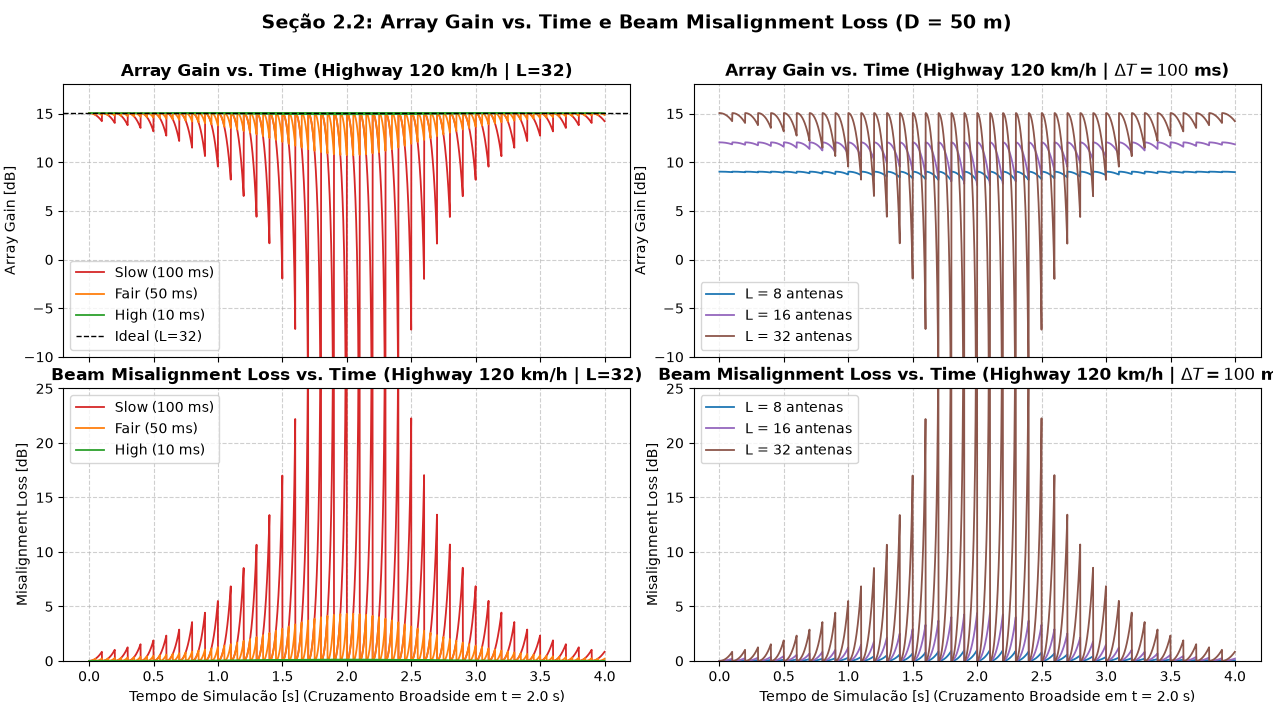
\includegraphics[width=0.98\linewidth]{Imagens/Activity02B.png} %
                \\ \footnotesize{\textit{Ganho do Arranjo e Desalinhamento em Highway ($120\text{ km/h}$, $D=50\text{ m}$).}} 
            \end{center}
        \end{column}
    \end{columns}
\end{frame}

\begin{frame}{Impacto da Velocidade e da Distância} 
    \begin{columns}
        \begin{column}{0.45\textwidth}
            \footnotesize{
            \textbf{1. Perfis de Mobilidade ($D = 50\text{ m}$):} 
            \begin{itemize}
                \item \textbf{Pedestrian ($3\text{ km/h}$):} Deslocamento de $8.3\text{ cm}$ por janela de $100\text{ ms}$ resulta em $0.00\text{ dB}$ de perda. 
                \item \textbf{Urban ($50\text{ km/h}$):} Oscilações moderadas no centro com picos de $\approx 3.2\text{ dB}$. 
                \item \textbf{Highway ($120\text{ km/h}$):} Picos instantâneos de até $70\text{ dB}$ nos nulos profundos de $L=32$. 
            \end{itemize}}
        \end{column}
        
        \begin{column}{0.55\textwidth}
            \begin{center}
                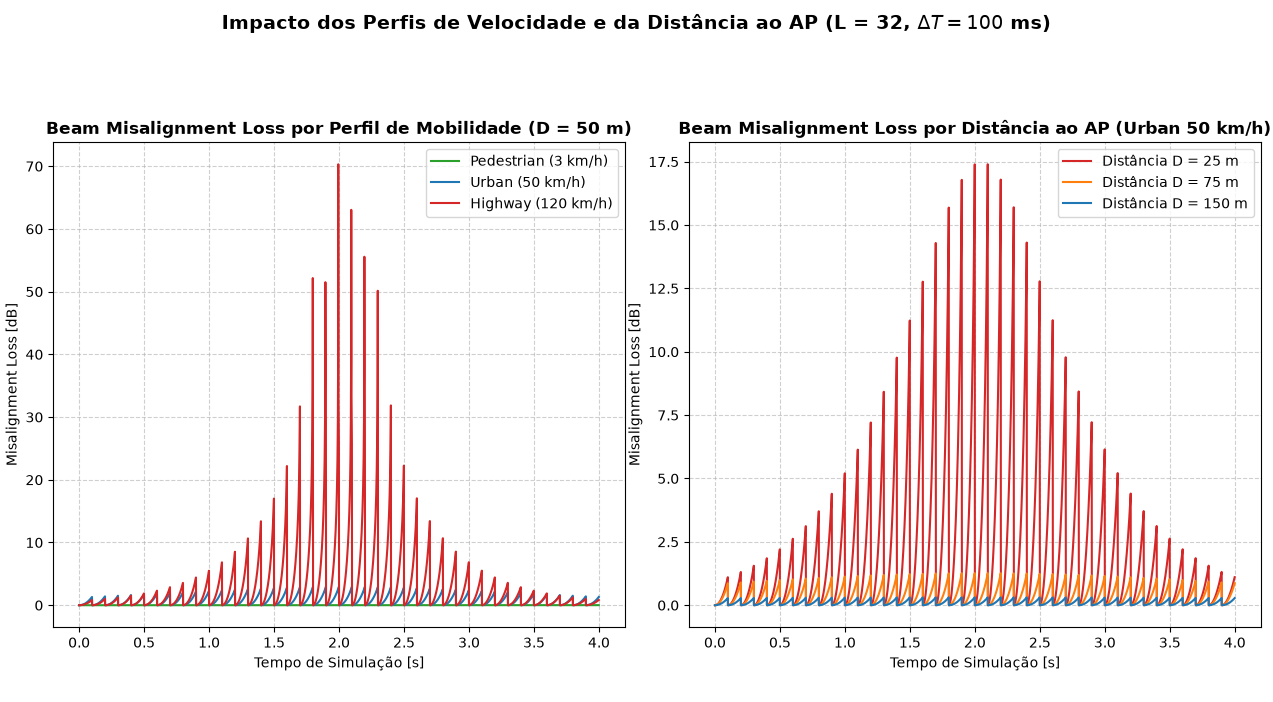
\includegraphics[width=0.98\linewidth]{Imagens/Activity02C.png} %
                \\ \footnotesize{\textit{Desalinhamento por velocidade e distância ($L=32$, $\Delta T = 100\text{ ms}$).}} 
            \end{center}
        \end{column}
    \end{columns}
\end{frame}

\begin{frame}{Impacto da Velocidade e da Distância} 
    \begin{columns}
        \begin{column}{0.45\textwidth}
            \footnotesize{
            \textbf{2. Distância ao AP ($50\text{ km/h}$):} 
            \begin{itemize}
                \item \textbf{Perto ($D = 25\text{ m}$):} Alta velocidade angular ($\omega_{\max} = v/D$) eleva a perda para $17.5\text{ dB}$. 
                \item \textbf{Meio/Borda ($75\text{ m}$ e $150\text{ m}$):} Variação angular suave reduz picos para $< 1.4\text{ dB}$ e $< 0.4\text{ dB}$. 
            \end{itemize}}
        \end{column}
        
        \begin{column}{0.55\textwidth}
            \begin{center}
                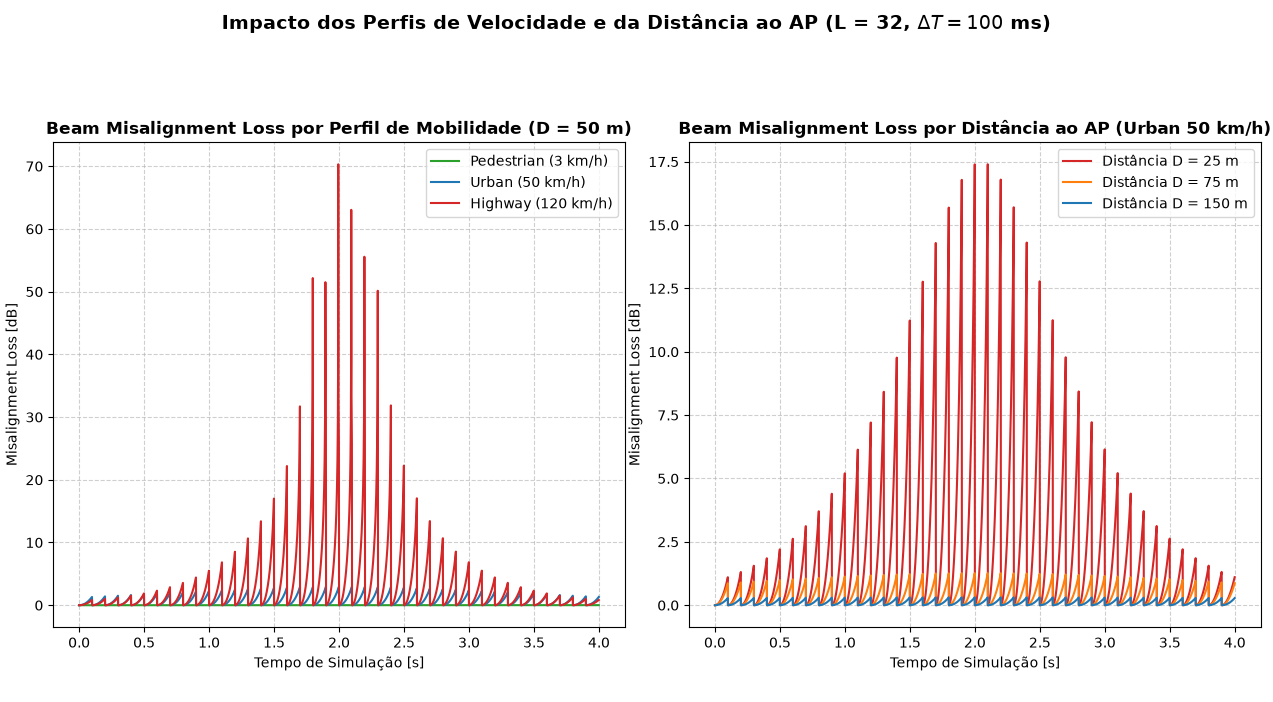
\includegraphics[width=0.98\linewidth]{Imagens/Activity02C.png} %
                \\ \footnotesize{\textit{Desalinhamento por velocidade e distância ($L=32$, $\Delta T = 100\text{ ms}$).}} 
            \end{center}
        \end{column}
    \end{columns}
\end{frame}

\begin{frame}{\textit{Trade-off}: Taxa de Atualização ($\Delta T$) vs. SE Líquida} 
    \begin{columns}
        \begin{column}{0.48\textwidth}
            \begin{table}
                \centering
                \resizebox{\textwidth}{!}{
                \begin{tabular}{l|c|ccc}
                    \hline
                    \textbf{Perfil} & \textbf{ULA} & \textbf{Slow ($100\text{ ms}$)} & \textbf{Fair ($50\text{ ms}$)} & \textbf{High ($10\text{ ms}$)} \\ 
                    & \textbf{($L$)} & \textbf{Perda | SE} & \textbf{Perda | SE} & \textbf{Perda | SE} \\ 
                    \hline
                    Pedestrian & 8  & 0.00 | \textbf{6.90} & 0.00 | 6.80 & 0.00 | 5.96 \\ 
                    ($3\text{ km/h}$) & 16 & 0.00 | \textbf{7.88} & 0.00 | 7.76 & 0.00 | 6.80 \\ 
                    & 32 & 0.00 | \textbf{8.87} & 0.00 | 8.73 & 0.00 | 7.65 \\ 
                    \hline
                    Urban & 8  & 0.04 | \textbf{6.63} & 0.01 | 6.54 & 0.00 | 5.73 \\ 
                    ($50\text{ km/h}$) & 16 & 0.18 | \textbf{7.56} & 0.04 | 7.49 & 0.00 | 6.57 \\ 
                    & 32 & 0.74 | 8.36 & 0.18 | \textbf{8.41} & 0.01 | 7.42 \\ 
                    \hline
                    Highway & 8  & 0.14 | \textbf{5.71} & 0.03 | 5.65 & 0.00 | 4.96 \\ 
                    ($120\text{ km/h}$) & 16 & 0.59 | 6.53 & 0.14 | \textbf{6.58} & 0.00 | 5.80 \\ 
                    & 32 & 3.08 | 6.75 & 0.59 | \textbf{7.39} & 0.02 | 6.64 \\ 
                    \hline
                \end{tabular}}
            \end{table}
            \vspace{-0.1cm}
            \scriptsize{
            \begin{itemize}
                \item \textbf{Baixa Mobilidade ($3\text{ km/h}$):} $\Delta T = 10\text{ ms}$ reduz a SE em $13.8\%$ por excesso de pilotos; \textbf{Slow ($100\text{ ms}$)} é ótimo ($8.87\text{ bps/Hz}$). 
                \item \textbf{Alta Mobilidade ($120\text{ km/h}$, $L=32$):} Em $100\text{ ms}$, a perda de $3.08\text{ dB}$ derruba a SE para $6.75\text{ bps/Hz}$. A taxa \textbf{Fair ($50\text{ ms}$)} recupera o alinhamento e atinge o pico de $\mathbf{7.39\text{ bps/Hz}}$. 
            \end{itemize}}
        \end{column}
        
        \begin{column}{0.52\textwidth}
            \begin{center}
                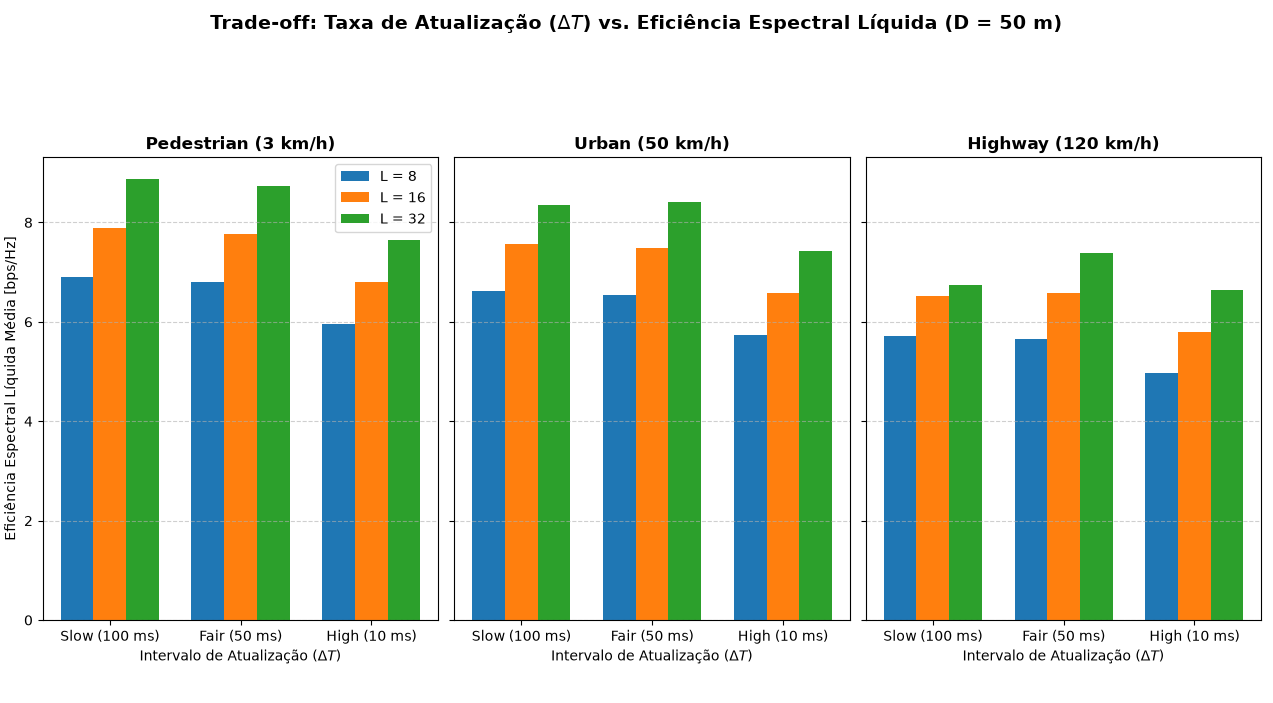
\includegraphics[width=0.98\linewidth]{Imagens/Activity02A.png} %
                \\ \footnotesize{\textit{Trade-off entre $\Delta T$ e Eficiência Espectral Líquida ($D = 50\text{ m}$).}} 
            \end{center}
        \end{column}
    \end{columns}
\end{frame}

% ======================================================= %
% SEÇÃO 3: CONCLUSÕES
% ======================================================= %
\section{Conclusões} 

\begin{frame}{Conclusões e Diretrizes de Projeto RRM} 
    \begin{block}{1. Otimização Conjunta \textit{Beamforming} + \textit{Dual-Loop PC}} 
        \begin{itemize}
            \item O acoplamento entre MRC e Controle de Potência em malha dupla elimina o gargalo de capacidade do DPC Fixo ($+30\%$ de \textit{Sum-Capacity} em $K=8$, entregando $26.38\text{ bps/Hz}$). 
            \item Garante a maior Eficiência Energética global ($406.27\text{ Mbits/Joule}$ em $K=8$) e reduz a taxa de \textit{Outage} frente ao regime \textit{Full Power} ($3.29\%$ vs. $4.32\%$). 
        \end{itemize}
    \end{block}

\end{frame}

\begin{frame}{Conclusões e Diretrizes de Projeto RRM} 
    \begin{block}{2. Rastreamento de Feixe Sensível ao Contexto Cinemático} 
        \begin{itemize}
            \item Arranjos \textit{Massive MIMO} ($L=32$) oferecem alto ganho direcional ($15.05\text{ dB}$), mas sofrem severa degradação sob atraso de atualização quando a velocidade angular ($\omega \propto v/D$) é elevada. 
            \item A periodicidade de treinamento de feixes ($\Delta T$) deve ser adaptada dinamicamente conforme a velocidade angular estimada e o tamanho do arranjo $L$, equilibrando precisão de apontamento e \textit{overhead} de sinalização. 
        \end{itemize}
    \end{block}
\end{frame}

\begin{frame}
    \begin{center}
        \Huge{\textbf{Obrigado!}}\\
        \vspace{0.4cm}
        \large{Apresentação Science Challenge 4A}\\ 
        \vspace{0.2cm}
        \normalsize{Mikael Ribeiro Camelo \& Caio Rodrigues} 
    \end{center}
\end{frame}

\end{document}